\documentclass{article}
\usepackage{graphicx}
\usepackage{amsmath}
% Note: composable package will be auto-injected by cstex

\title{CSF Declarative - Clean Annotations}
\author{CSF Team}
\date{\today}

\begin{document}

\maketitle

\section{Introduction}

This document demonstrates the **clean** CSF Declarative approach where users provide
minimal semantic hints and CSTeX automatically surfaces all the detailed metadata.

\section{Statistical Results}

% CSF-STAT: name=main_correlation, type=correlation
Our analysis revealed a strong correlation between temperature and pressure 
(r = \csfstatlink{main_correlation}{float,round2}).

% CSF-STAT: name=significance_test, type=p_value  
This correlation is statistically significant (p < \csfstatlink{significance_test}{scientific,round3}).

% CSF-COMPUTE: name=sample_mean, expr="np.mean(data.temperature)"
The mean temperature was \csfstatlink{sample_mean}{float,round1}°C across all measurements.

% CSF-COMPUTE: name=model_accuracy, expr="model.score(X_test, y_test)"
Our predictive model achieved an accuracy of \csfstatlink{model_accuracy}{percent,round1} on the test dataset.

\section{Figures}

% CSF-ARTIFACT: type=figure, path=figures/temperature_measurement.png
\begin{figure}[h]
\centering
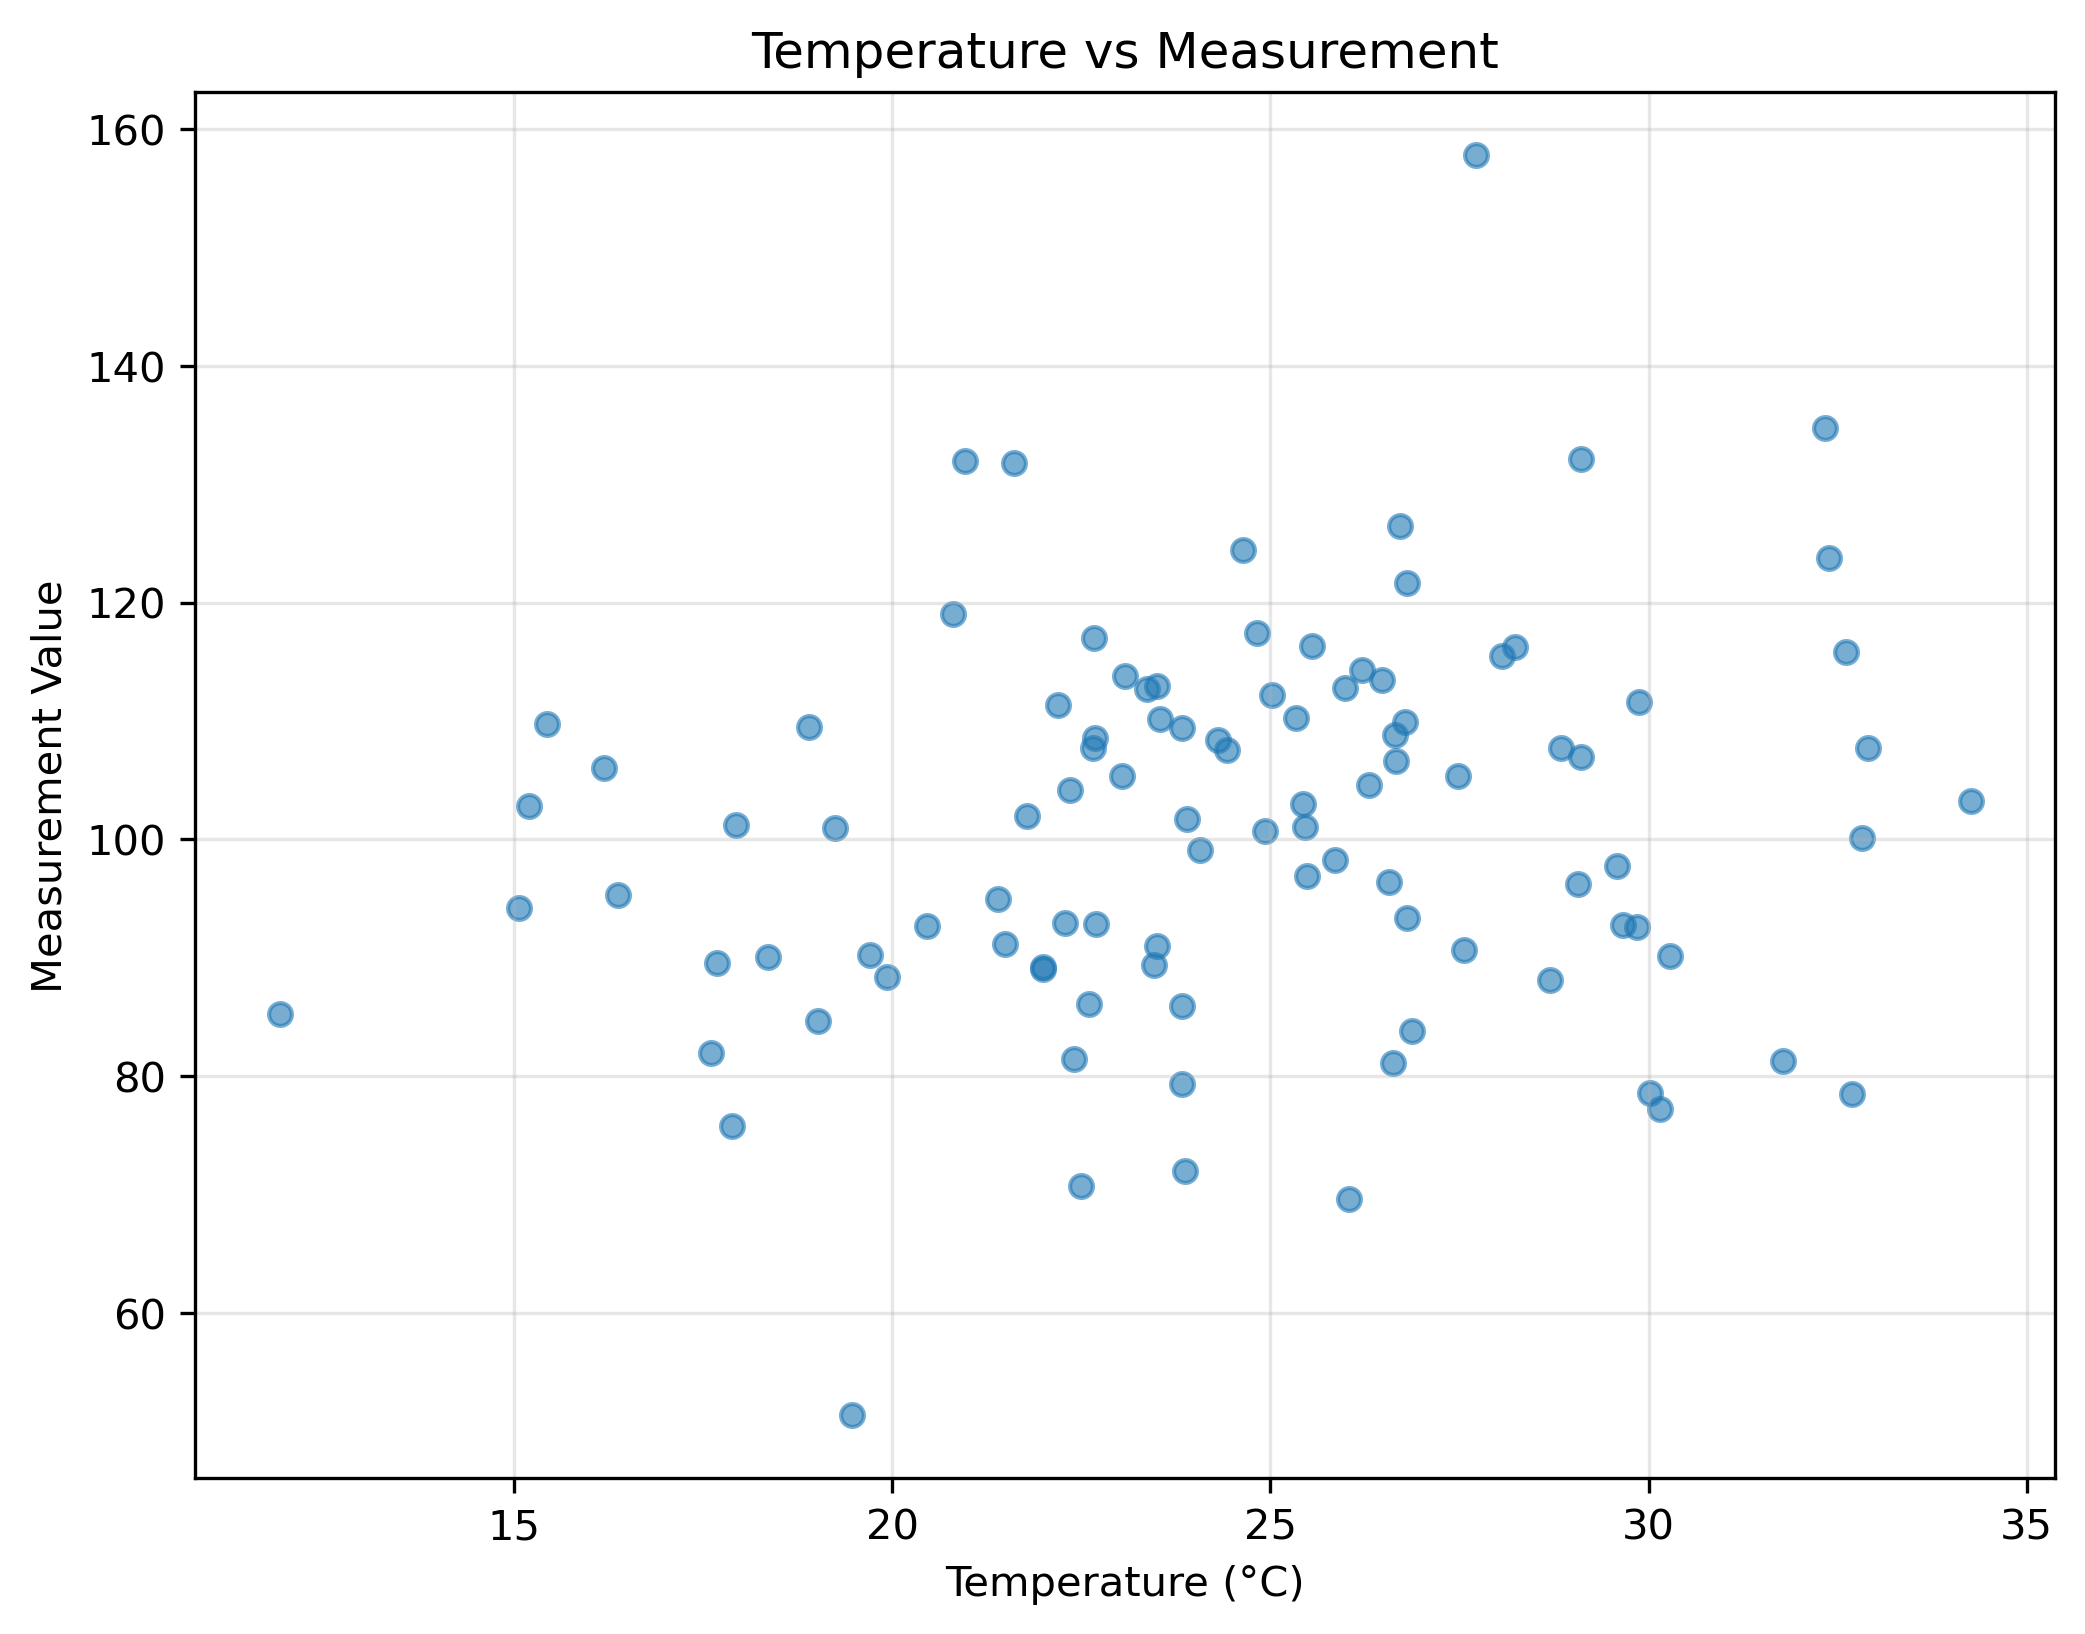
\includegraphics[width=0.8\textwidth]{figures/temperature_measurement.png}
\caption{Temperature vs Measurement Analysis}
\label{fig:temp}
\end{figure}

The figure above (\ref{fig:temp}) uses minimal CSF metadata - CSTeX will automatically 
discover which script generated it, at what line, and from which pipeline step.

\section{Data Tables}

% CSF-TABLE: path=outputs/summary_stats.csv
\begin{table}[h]
\centering
\begin{tabular}{|l|r|r|}
\hline
Statistic & Value & Unit \\
\hline
Mean Temperature & 23.7 & °C \\
Std Deviation & 4.2 & °C \\
Sample Size & 1000 & measurements \\
\hline
\end{tabular}
\csftablelink{outputs/summary_stats.csv}{auto}
\caption{Summary statistics}
\label{tab:summary}
\end{table}

Table \ref{tab:summary} shows summary statistics. The CSTeX compiler will automatically
determine that this comes from the summarization step, generated by scripts/summarize.py.

\section{Mixed Automatic and Declarative}

% Automatic discovery - no annotation needed
\begin{figure}[h]
\centering
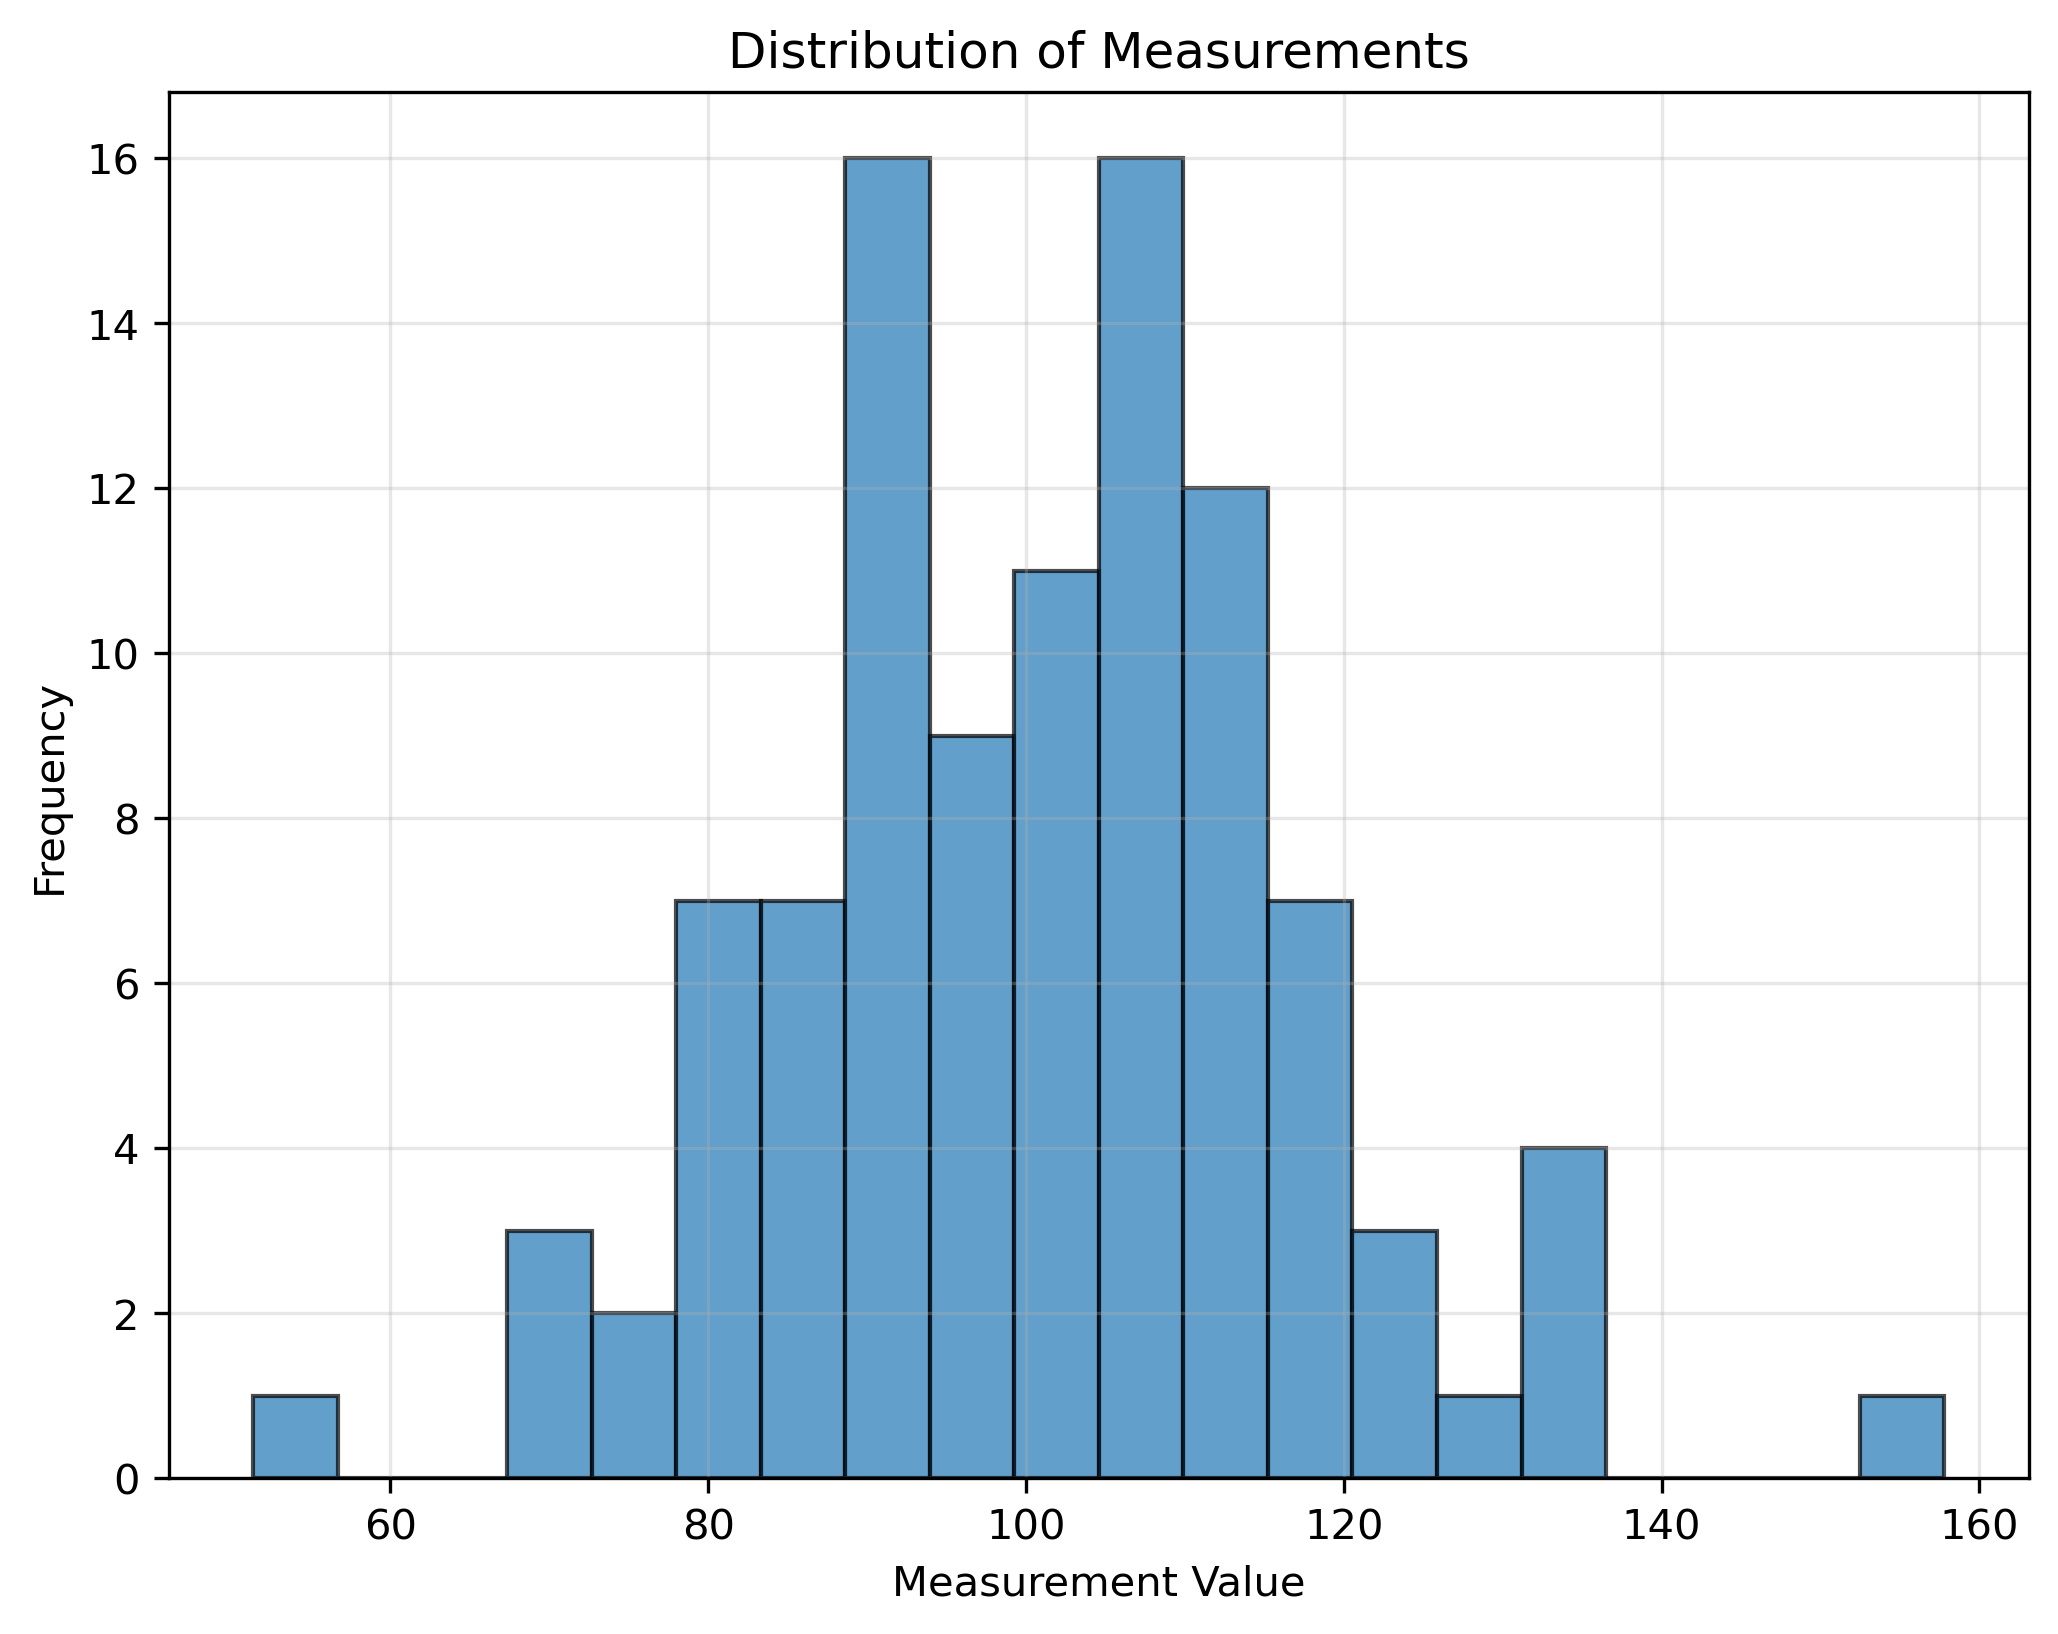
\includegraphics[width=0.7\textwidth]{figures/measurement_distribution.png}
\caption{Distribution plot discovered automatically}
\label{fig:auto}
\end{figure}

% Minimal declarative annotation when automatic discovery is insufficient
% CSF-ARTIFACT: type=figure, path=figures/custom_analysis.png  
\begin{figure}[h]
\centering
\includegraphics[width=0.7\textwidth]{figures/custom_analysis.png}
\caption{Custom analysis requiring minimal semantic hint}
\label{fig:custom}
\end{figure}

Figure \ref{fig:auto} uses automatic discovery, while Figure \ref{fig:custom} uses 
a minimal declarative annotation. In both cases, CSTeX will surface the complete
metadata automatically.

\section{Key Benefits}

\subsection{Clean Source Documents}
Users write minimal, semantic annotations:
\begin{itemize}
    \item \texttt{\% CSF-STAT: name=correlation, type=correlation}
    \item \texttt{\% CSF-COMPUTE: name=accuracy, expr="model.score(X\_test, y\_test)"}
    \item \texttt{\% CSF-ARTIFACT: type=figure, path=figures/plot.png}
\end{itemize}

\subsection{Automatic Metadata Surfacing}
CSTeX automatically discovers and injects:
\begin{itemize}
    \item Which script generated each artifact
    \item Exact line numbers in source code
    \item Pipeline step dependencies
    \item Computational context and provenance
\end{itemize}

\subsection{Plain LaTeX Compatibility}
\begin{itemize}
    \item CSF comments are invisible to plain LaTeX
    \item Fallback commands show format specifiers
    \item No vendor lock-in or special requirements
\end{itemize}

\section{Conclusion}

This approach provides the best developer experience:
\begin{enumerate}
    \item \textbf{Minimal annotations} - Users provide just semantic hints
    \item \textbf{Automatic surfacing} - CSTeX discovers all detailed metadata
    \item \textbf{Clean source} - No manual metadata maintenance required
    \item \textbf{Full transparency} - Complete computational provenance
\end{enumerate}

The result is computational transparency without the burden of manual metadata management.

\end{document}